% !TEX root = ../eval.tex

\section{Methods}%
\label{sec:data}

While we were unable to pre-register the analysis because we have had access to
and been working with the Money Dashoard data for months, we proceeded in the
same spirit: we first wrote a draft of the paper in the form of a pre-analysis
plan, following \citet{olken2015promises}, then tested the entire code base --
data pre-processing, balance checks, main analysis, and extensions -- with a 1
percent sample, and finally ran the entire analysis.


\subsection{Dataset}%
\label{sub:dataset}

\begin{itemize}

    \item Money Dashboard can access up to three years of historic data for
        each account a user links to their account.

    \item Each user for whom we have sufficient data thus serves as both a
        treatment unit and a potential control unit.

    \item Limitations: We have more data for users that signed up later. So average user in
        the study is not the average MDB user. If time of signup is mainly
        driven by financial savyness, then study sample is closer to overall
        population than MDB sample (if we rank groups as early joiners > late
        joiners > never joiners in terms of financial sophistication). If,
        however, signup reflects something like openness to newness, then it's
        not necessarily correlated with financial savyness. Either way, we
        might ignore it for now. We could test whether behaviour differs
        between early or late adopters, but that doesn't seem important enough.

\end{itemize}


\subsection{Sample selection and data preprocessing}%
\label{sub:sample_selection}

To assess the impact of app use on users' financial behaviour we need to
observe their relevant financial history for a sufficiently long period of time
prior to and after signup. For our purpose here, ``relevant
financial history'' includes the complete set of spending transactions and all
savings account inflows and outflows, and ``sufficiently long period'' is a
period of 6 months prior to and after signup, with the month of signup being
the first month of the latter period.\footnote{In
Appendix~\ref{sub:alternative_matching_method} we show results with different
window lengths. \edit{The results are unchanged.}}

Table~\ref{tab:selection} provides an overview of the precise conditions we applied to implement
these criteria and their effect on the sample size. The set of functions that
implement each condition can be found on \href{path-to-github}{path to github}.

\begin{table}
\centering
\caption{Sample selection}\label{tab:selection}
\begin{tabular}{lrrrr}
\toprule
                                       &  Users & User-months &       Txns & Txns (m\pounds) \\
\midrule
                            Raw sample & 27,329 &     803,012 & 67,088,876 &          12,722 \\
Annual income of at least \pounds5,000 &  9,338 &     256,891 & 24,582,995 &           4,463 \\
          At least one savings account &  5,579 &     167,705 & 16,952,445 &           3,249 \\
            At least 12 months of data &  4,884 &     163,602 & 16,657,929 &           3,207 \\
  Monthly spend of at least \pounds200 &  2,506 &      82,860 &  9,303,691 &           1,823 \\
                          Final sample &  2,506 &      82,860 &  9,303,691 &           1,823 \\
\bottomrule
\end{tabular}

\tabnote{\textwidth}{Number of users, user-months, transactions, and
transaction volume in millions of British Pounds left in our sample after each sample selection step. Link to sample selection
code:
\href{https://github.com/fabiangunzinger/mdb_eval/blob/main/src/data/selectors.py}{\faGithub}.}
\end{table}

\paragraph{Data transformations}%
\label{par:data_transformations}

To minimise the influence of outliers, we winsorise spend, income, and savings
accounts flow variables at the 5 percent level or -- if we winsorise on both
ends of the distribution -- at the 2.5 percent level.

\edit{Question: how to determine winsor level? Currently using 5 percent
because 1 percent still leaves very large values in the data: 20k spend, 15k
income, 20k sa inflows/outflows, all per user-month}





\subsection{Summary statistics}%
\label{sub:summary_statistics}

Figure~\ref{fig:sample_description} describes the sample.

\begin{figure}[htpb]
    \centering
    \caption{Sample description}%
    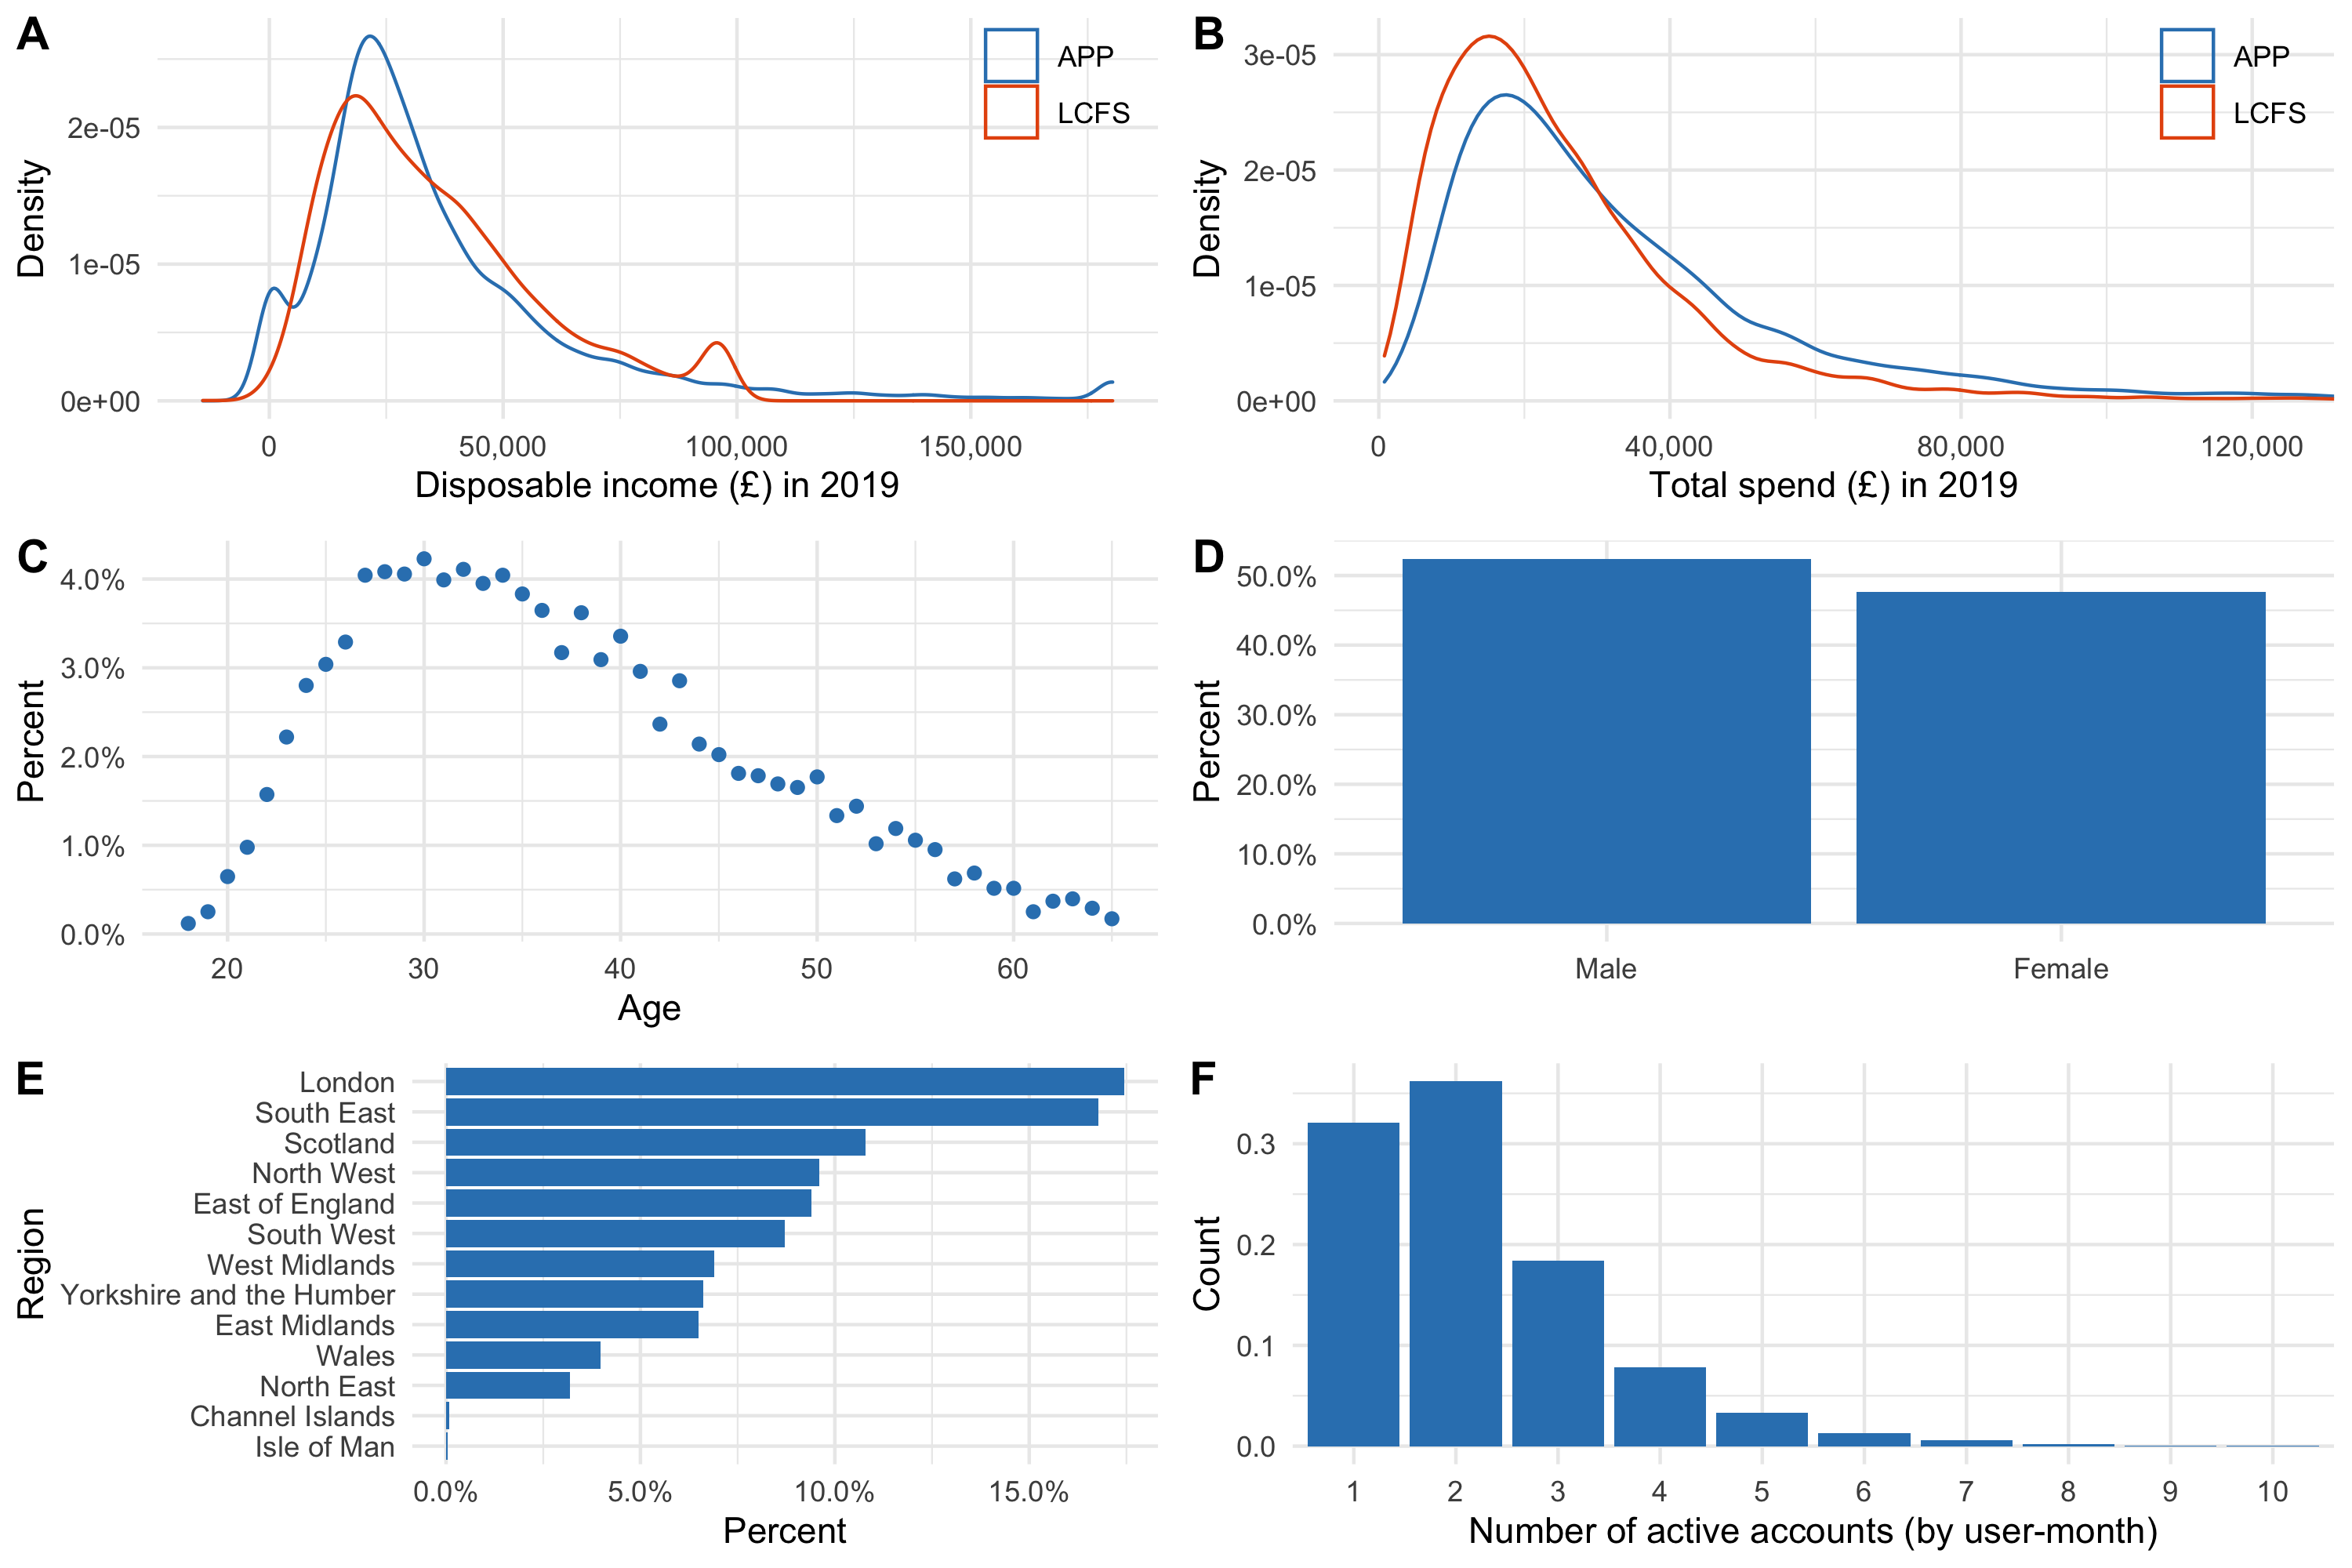
\includegraphics[width=0.8\linewidth]{\figdir/sample_description.png}
    \label{fig:sample_description}
    \fignote{\textwidth}{}
\end{figure}

Table~\ref{tab:sumstats} provides summary statistics.


\begin{table}[htbp]
   \centering
   \tiny
   \begin{threeparttable}[b]
      \caption{\label{tab:reg_compare} Regression results}
      \begin{tabular}{lcccccc}
         \tabularnewline \midrule \midrule
         Dependent Variable: & \multicolumn{6}{c}{Net-inflows}\\
         Model:                     & (1)                   & (2)                & (3)                & (4)                & (5)               & (6)\\  
         \midrule
         \emph{Variables}\\
         App use                    & 14.330$^{**}$         & 15.303$^{***}$     & 15.303$^{***}$     & 19.381$^{***}$     & 15.963$^{**}$     & 20.207$^{***}$\\   
                                    & [2.650; 26.009]       & [3.686; 26.919]    & [3.686; 26.919]    & [7.110; 31.652]    & [1.881; 30.045]   & [7.940; 32.473]\\   
         Month income               &                       & 0.053$^{***}$      & 0.053$^{***}$      & 0.060$^{***}$      & 0.053$^{***}$     & 0.058$^{***}$\\   
                                    &                       & [0.049; 0.058]     & [0.049; 0.058]     & [0.045; 0.075]     & [0.045; 0.060]    & [0.043; 0.073]\\   
         Month spend                &                       & -0.077$^{***}$     & -0.077$^{***}$     & -0.100$^{***}$     & -0.076$^{***}$    & -0.098$^{***}$\\   
                                    &                       & [-0.081; -0.073]   & [-0.081; -0.073]   & [-0.109; -0.091]   & [-0.091; -0.061]  & [-0.107; -0.089]\\   
         Disc. spend                &                       & 138.940$^{***}$    & 138.940$^{***}$    & 169.002$^{***}$    & 132.862$^{***}$   & 156.441$^{***}$\\   
                                    &                       & [115.597; 162.282] & [115.597; 162.282] & [128.874; 209.129] & [90.975; 174.750] & [115.907; 196.976]\\   
         Female                     &                       & -14.521$^{***}$    & -14.521$^{***}$    &                    & -14.247$^{***}$   &   \\   
                                    &                       & [-24.998; -4.044]  & [-24.998; -4.044]  &                    & [-21.206; -7.289] &   \\   
         Generation $=$ GenX        &                       & 39.071$^{***}$     & 39.071$^{***}$     &                    & 39.379$^{**}$     &   \\   
                                    &                       & [19.258; 58.885]   & [19.258; 58.885]   &                    & [9.611; 69.148]   &   \\   
         Generation $=$ Millennials &                       & 71.330$^{***}$     & 71.330$^{***}$     &                    & 71.699$^{***}$    &   \\   
                                    &                       & [51.964; 90.697]   & [51.964; 90.697]   &                    & [40.338; 103.060] &   \\   
         Generation $=$ GenZ        &                       & 42.302             & 42.302             &                    & 43.095$^{*}$      &   \\   
                                    &                       & [-9.381; 93.985]   & [-9.381; 93.985]   &                    & [-7.002; 93.192]  &   \\   
         Intercept                  & -20.523$^{***}$       & -59.208$^{***}$    & -59.208$^{***}$    &                    &                   &   \\   
                                    & [-30.679; -10.368]    & [-84.179; -34.237] & [-84.179; -34.237] &                    &                   &   \\   
         \midrule
         \emph{Fixed-effects}\\
         User FE                    &                       &                    &                    & Yes                &                   & Yes\\  
         Month FE                   &                       &                    &                    &                    & Yes               & Yes\\  
         \midrule
         \emph{Fit statistics}\\
         Observations               & 184,847               & 184,847            & 184,847            & 184,847            & 184,847           & 184,847\\  
         R$^2$                      & $3.13\times 10^{-5}$  & 0.01132            & 0.01132            & 0.10137            & 0.01203           & 0.10203\\  
         Within R$^2$               &                       &                    &                    & 0.00905            & 0.01117           & 0.00885\\  
         \midrule \midrule
         \multicolumn{7}{l}{\emph{Signif. Codes: ***: 0.01, **: 0.05, *: 0.1}}\\
      \end{tabular}
   \end{threeparttable}
\end{table}





\subsection{Treatment}%
\label{sub:treatment}

A user changes treatment status from untreated to treated when they start using
the app. Figure~\ref{fig:treatplot_sample_raw} shows the treatment history for
200 randomly selected users.

\begin{figure}[htpb]
    \centering
    \caption{Treatment assignment plot}%
    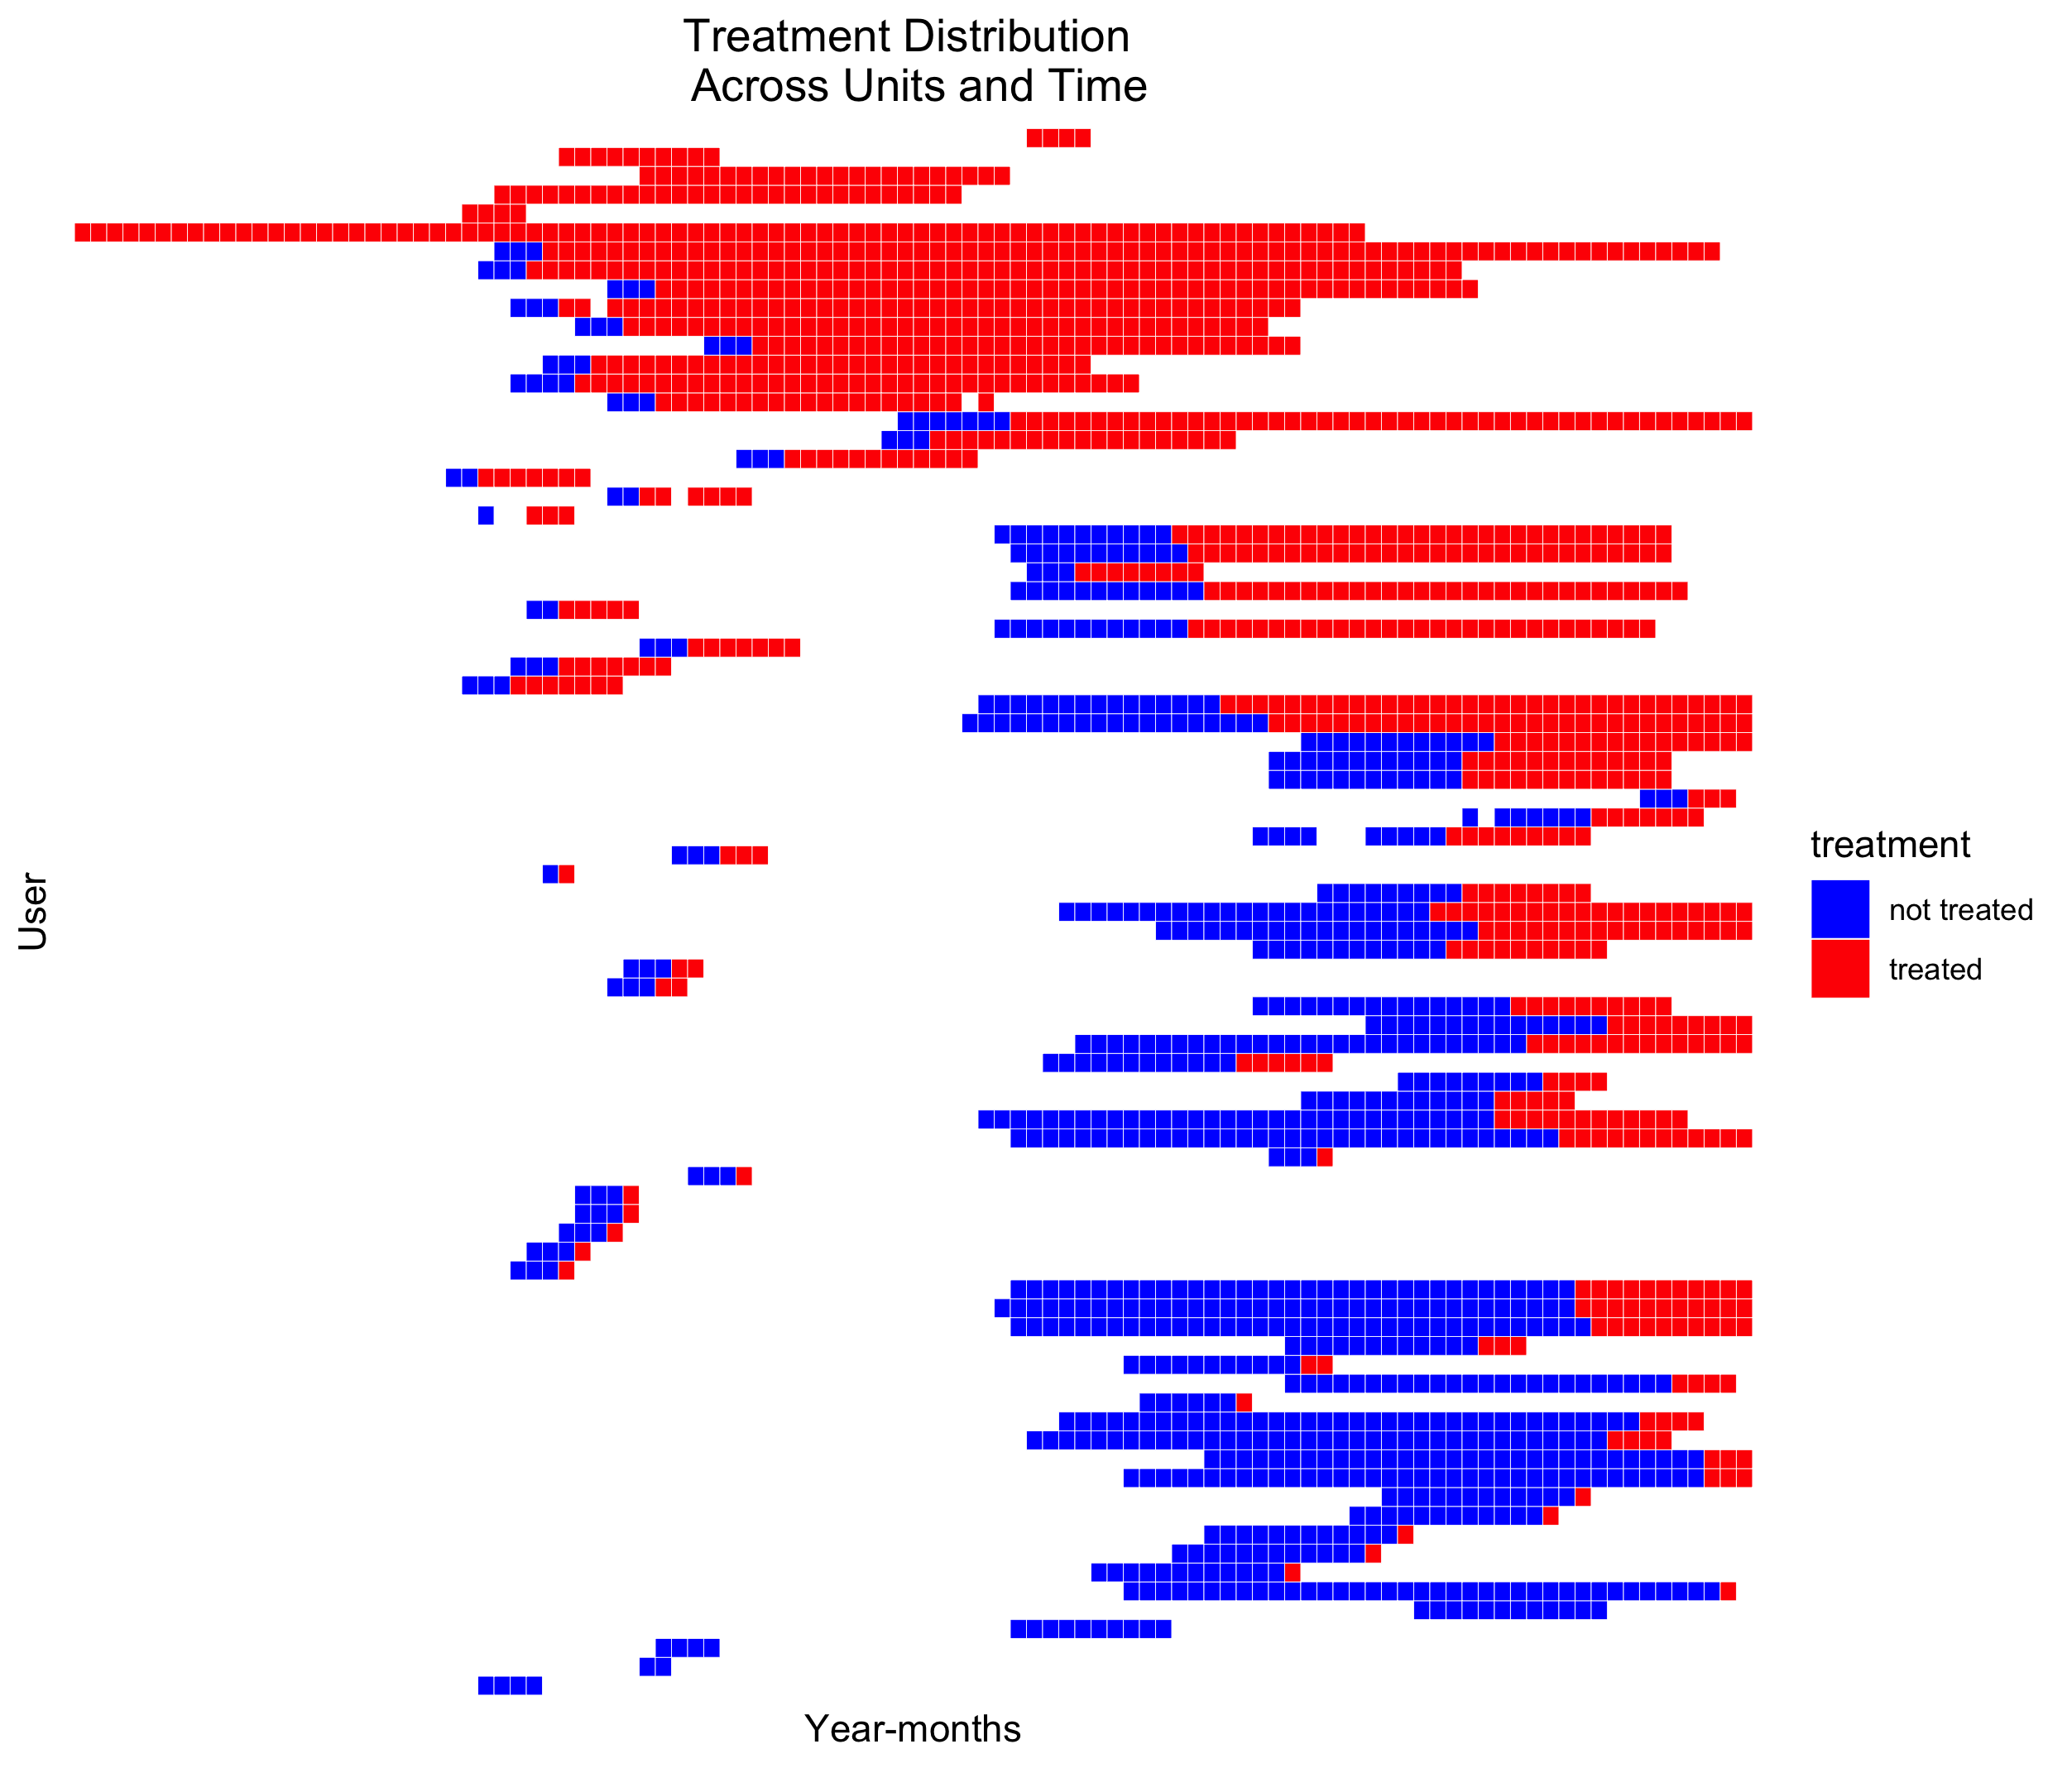
\includegraphics[width=0.8\linewidth]{\figdir/treatplot_sample_raw.png}
    \label{fig:treatplot_sample_raw}

    \fignote{\textwidth}{Each horizontal line shows for one of 200 randomly
        selected users the observed pre and post signup periods in blue and
        red, respectively. The faint vertical white lines indicate month
        borders, whitespace indicates periods in which we do not observe the
    user. To the left of the observed period, this is because the app cannot
access data before that point when the user signs up; to the right, because
they have stopped using the app.}

\end{figure}


\subsection{Outcomes}%
\label{sub:outcomes}

Savings... see Table~\ref{tab:vars} for details.

For a more nuanced understanding of how app use affects savings we also
consider net-savings -- total savings account inflows minus outflows -- as a
proportion of monthly income to see whether a willingness to save more might be
offset by a (later) need to withdraw funds, and a dummy variable for whether a
user has any savings account inflows in a given month to see whether the app
helps users save at all. To investigate possible channels, we consider total
spend, highly discretionary spend, banking charges, the total amount of
borrowing, as well as payday borrowing, all as proportion of monthly income.

\paragraph{Adjusting for multiple hypothesis tests}%
\label{par:adjusting_for_multiple_hypothesis_tests}
We think of our secondary outcomes as exploratory and do not make any
adjustments for multiple hypothesis testing.\footnote{For a recent
game-theoretically motivated discussion of when and how to correct for multiple
hypothesis testing, see \citet{viviano2021should}.} An alternative approach,
based on \citet{anderson2008multiple}, would be to group outcomes into
``savings'', ``spending'', ``borrowing'', and ``fees'', and consider them as
different dimensions of a latent variable of interest which we might call
``financial management skills''. We do not do that for two reasons: first and
foremost, because we think it is natural to think of the amount saved as the
ultimate outcome and of other outcomes as providing a more nuanced
understanding of savings behaviour or as suggesting possible channels through
which app use affects savings. Thinking of savings as the main goal is also
reflected in Money Dashboard's main promise, which is to help users spend less
and save more, as shown in Figure~\ref{fig:mdb_website}. Second, as pointed out
in \citet{carlin2017fintech}, incurring overdraft fees is not an unambiguous
sign of a financial mistake, as the opportunity to go into overdraft confers a
benefit to the consumer.\footnote{For further discussions on fees, see
\citet{jorring2020financial, stango2009consumers}.}


\subsection{Covariates}%
\label{sub:covariates}

We control for baseline behaviour, events, and personal characteristics that,
to various degrees, capture a person's need, capacity, motivation, and
awareness to save. Table~\ref{tab:vars} lists all covariates used
together with their definition and the rationale for including them. For all
variables, we include contemporaneous values as well as lags for up to 6
periods. In addition, we control for the previous six months of savings to
capture time-invariant unobserved drivers of savings behaviour (in
specifications without fixed effects) as well as a possible signal for a higher
or lower need for future savings.

Following \citet{vanderweele2019principles} we include covariates that affect
either outcomes or the propensity for treatment or both, exclude from this
set of variables those that are instruments (affect the outcome only through their effect on
treatment propensity) and add to it proxies for unobserved variables that are a
common cause of both outcomes and treatment propensity.\footnote{
\citet{vanderweele2019principles} calls this the ``modified disjunctive cause
criterion'' for covariate selection, as it includes the set of variables that are causally
related to either outcomes, or treatment propensity, or both, but modified to
account for potential bias by excluding instruments and including proxies of
unobserved causes of both outcomes and treatment.}

\subsection{Estimation}%
\label{sub:difference_in_difference}

Control group design:
\begin{itemize}

    \item We only have data for a self-selected group of people who choose to
        use the app. This has a couple consequences:

    \item By virtue of signing up to an app that helps them manage
        their money, these users are different from those who don't
        sign up. As a result, we are unable to answer the question of
        whether app use helps the average person in the
        population as a whole save more.\footnote{One way to get closer
            to that answer is to re-weight our sample on observable
            demographic variables so as to match the UK population as a
            whole. But our sample differs from the population as a
            whole both is ways that are observable (demographic
            variables) and unobservable (self-awareness that they need
            help managing their money, cognitive resources to engage
            with the app, motivation to do so). Re-weighting would only
            help us deal with the first of these.}

    \item Even among people who do eventually sign up to the app,
        hte decision when to do so is unlikely to be random --
        \textit{something} makes them sign up at the particular
        point in time they do and not before or after. If we think
        of this factor as ``motivation to save more'', then said
        motivation is inextricably linked with the decision to sign
        up so that we cannot differentiate between the two.

    \item Hence: due to the first point above, we cannot estimate
        an ATE (effect of app use on the average citizen), and due
        to the second point we also cannot estimate a pure ATT
        (effect of app use on users). Instead, our estimated effect
        of app use captures the effect of being motivated to save
        more and using the app to do so.\footnote{One way to get a
            step closer to ATT would be to find a variable that
        correlates with ``motivation to save'' and control for it /
    match on it.}

    \item This is true for both our matched DiD and our TWFE
        design. While these two approaches use a different
        counterfactual to estimate the effect of app use
        (behaviour of a matched control in the case of DiD and
        extrapolating within-user pre-signup behaviour in the case
        of TWFE), neither can help us with the fact that the
        decision to sign up is likely correlated with the
        time-varying unobserved effect ``motivation to save more''.

\end{itemize}

DiD:
\begin{itemize}

    \item We use a difference-in-differences design to estimate the effect of
        app use. Because we do not have a separate control group, we use the
        per-signup data of Money Dashboard users as control periods and use
        matching to find comparable control user for each tretment user.

    \item To do this, we use the matching estimator for panel data proposed by
        \citet{imai2021matching}. Following paper, we conduct the following
        steps:

    \item For each treated observation, we find a set of control observations
        with that share the same treatment history for a period of $L$ periods
        before the treatment and $F$ periods after the treatment. In our
        baseline specification, we rely on a year's worth of data around the
        treatment period and set $L=6$ and $F = 0, 1, 2, 3, 4, 5$.

    \item Identification assumption is that potential outcomes only depend on
        treatment status of the past L periods. In general, this means that if
        treatment has a cumulative effect over time, the full effect is reached
        after L periods. In our context, this means that any effect on savings
        behaviour from usign the app is fully realised after L periods. (I
        think this means that if we look at the treatment effect for F periods
        forward, the effect should not become stronger after F = L).

\end{itemize}

DiD identification assumptions:
\begin{itemize}
    \item No spillover effects: the potential outcome of unit $i$ at time $t$
        is independent of the treatment status of other units. This is violated
        if a user's partner or friends also use the app and, through sharing
        their experiences or motivations, influence the user's savings
        behaviour.

    \item Carryover effects no longer than $L$ periods: a user's potential
        outcome in period $t$ is independent of treatment status in periods
        more than $L$ periods ago. Given that we are dealing with an absorbing
        treatment, this is not a very strong assumption in our context, and we
        choose $L$ based on what we think is an informative number of periods
        to observe pre-app use behaviour.\footnote{An absorbing treatment is
            one that cannot be reversed, and hence we only change from
            untreated to treated once.}.

    \item Parallel trends: the spending trajectory between treated and control
        units would have continued to be parallel if the treated unit hadn't
        started using the app. This is violated whenever an intended change in
        savings behaviour also provided the impetus for the user to start using
        the app, which is likely to occurr frequently. To the extent this is
        the case, we have an ommitted variable ``motivation to save more'',
        which both changes the user's savings behaviour and their treatment
        status. Because of this, what we are measuring is not a pure ATT of app
        use -- the effect of app use on savings over and above the change
        precipitated by a change motivation -- but the effect of app use for
        users motivated to save more.

\end{itemize}


\begin{figure}[htpb]
    \centering
    \caption{Match set examples}%
    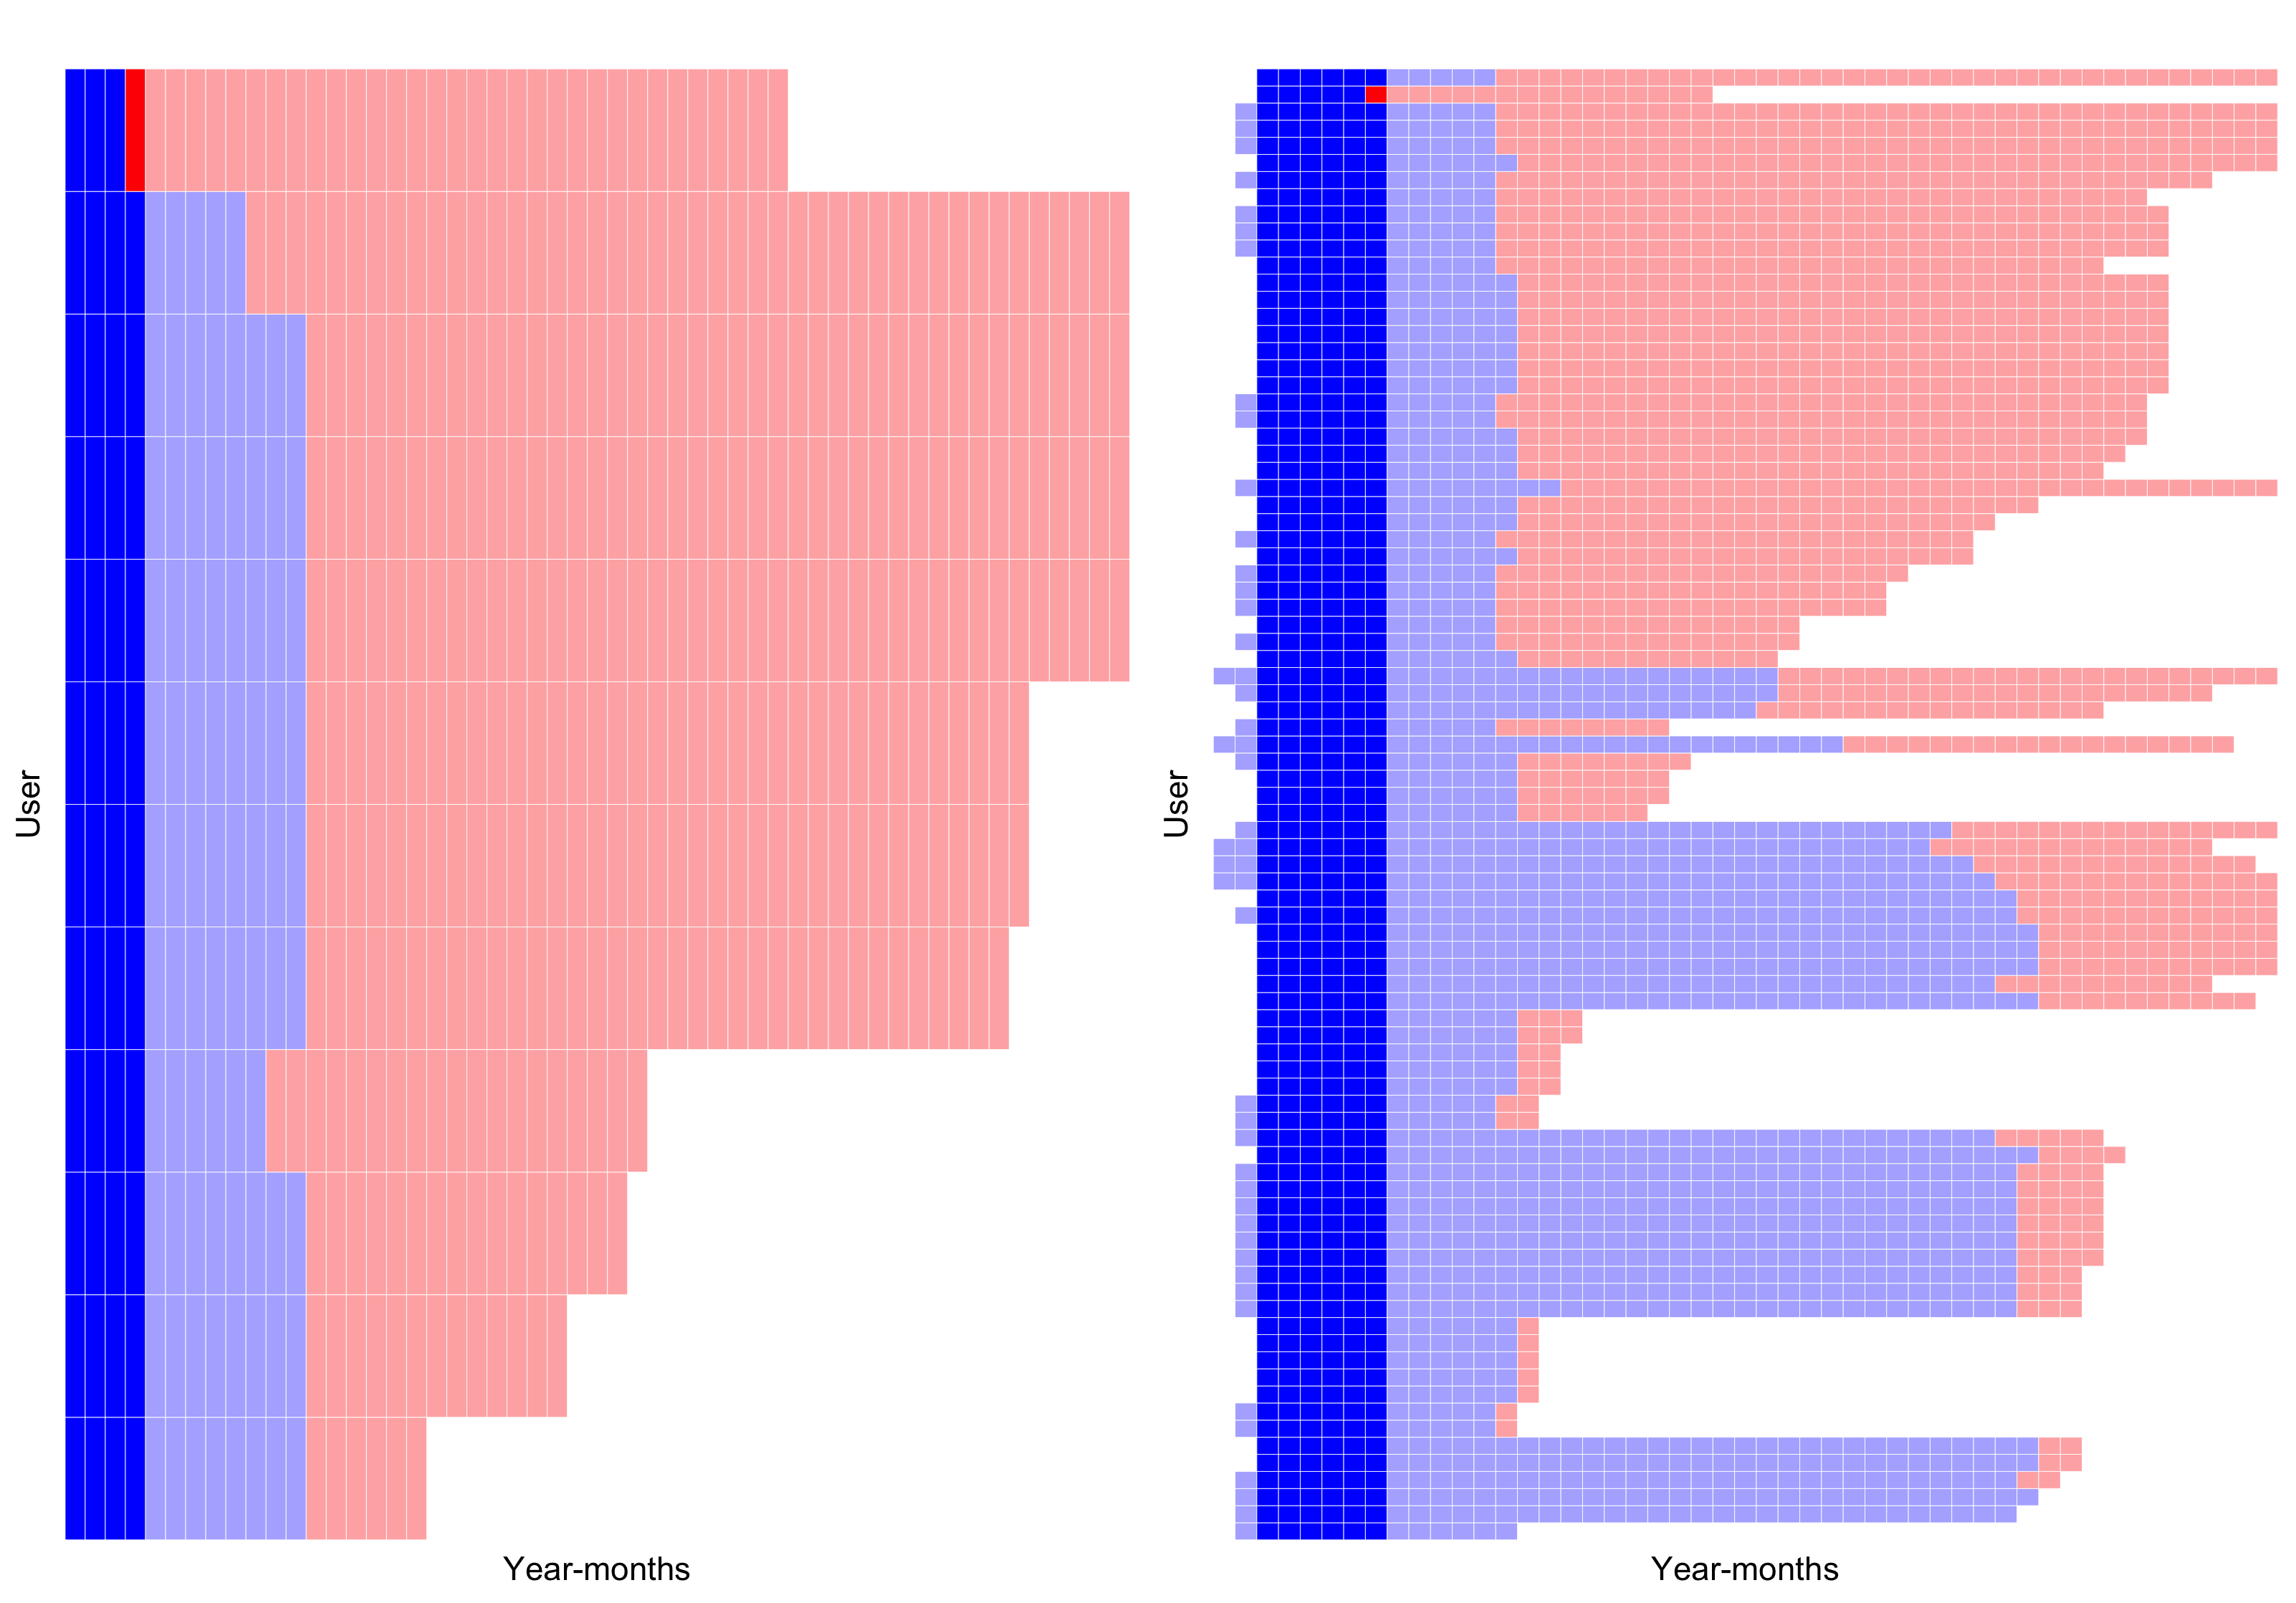
\includegraphics[width=\linewidth]{\figdir/matchset_examples.png}
    \label{fig:matchset_examples}

    \fignote{\textwidth}{}

\end{figure}


\begin{figure}[htpb]
    \centering
    \caption{Distribution of size of matched control units}%
    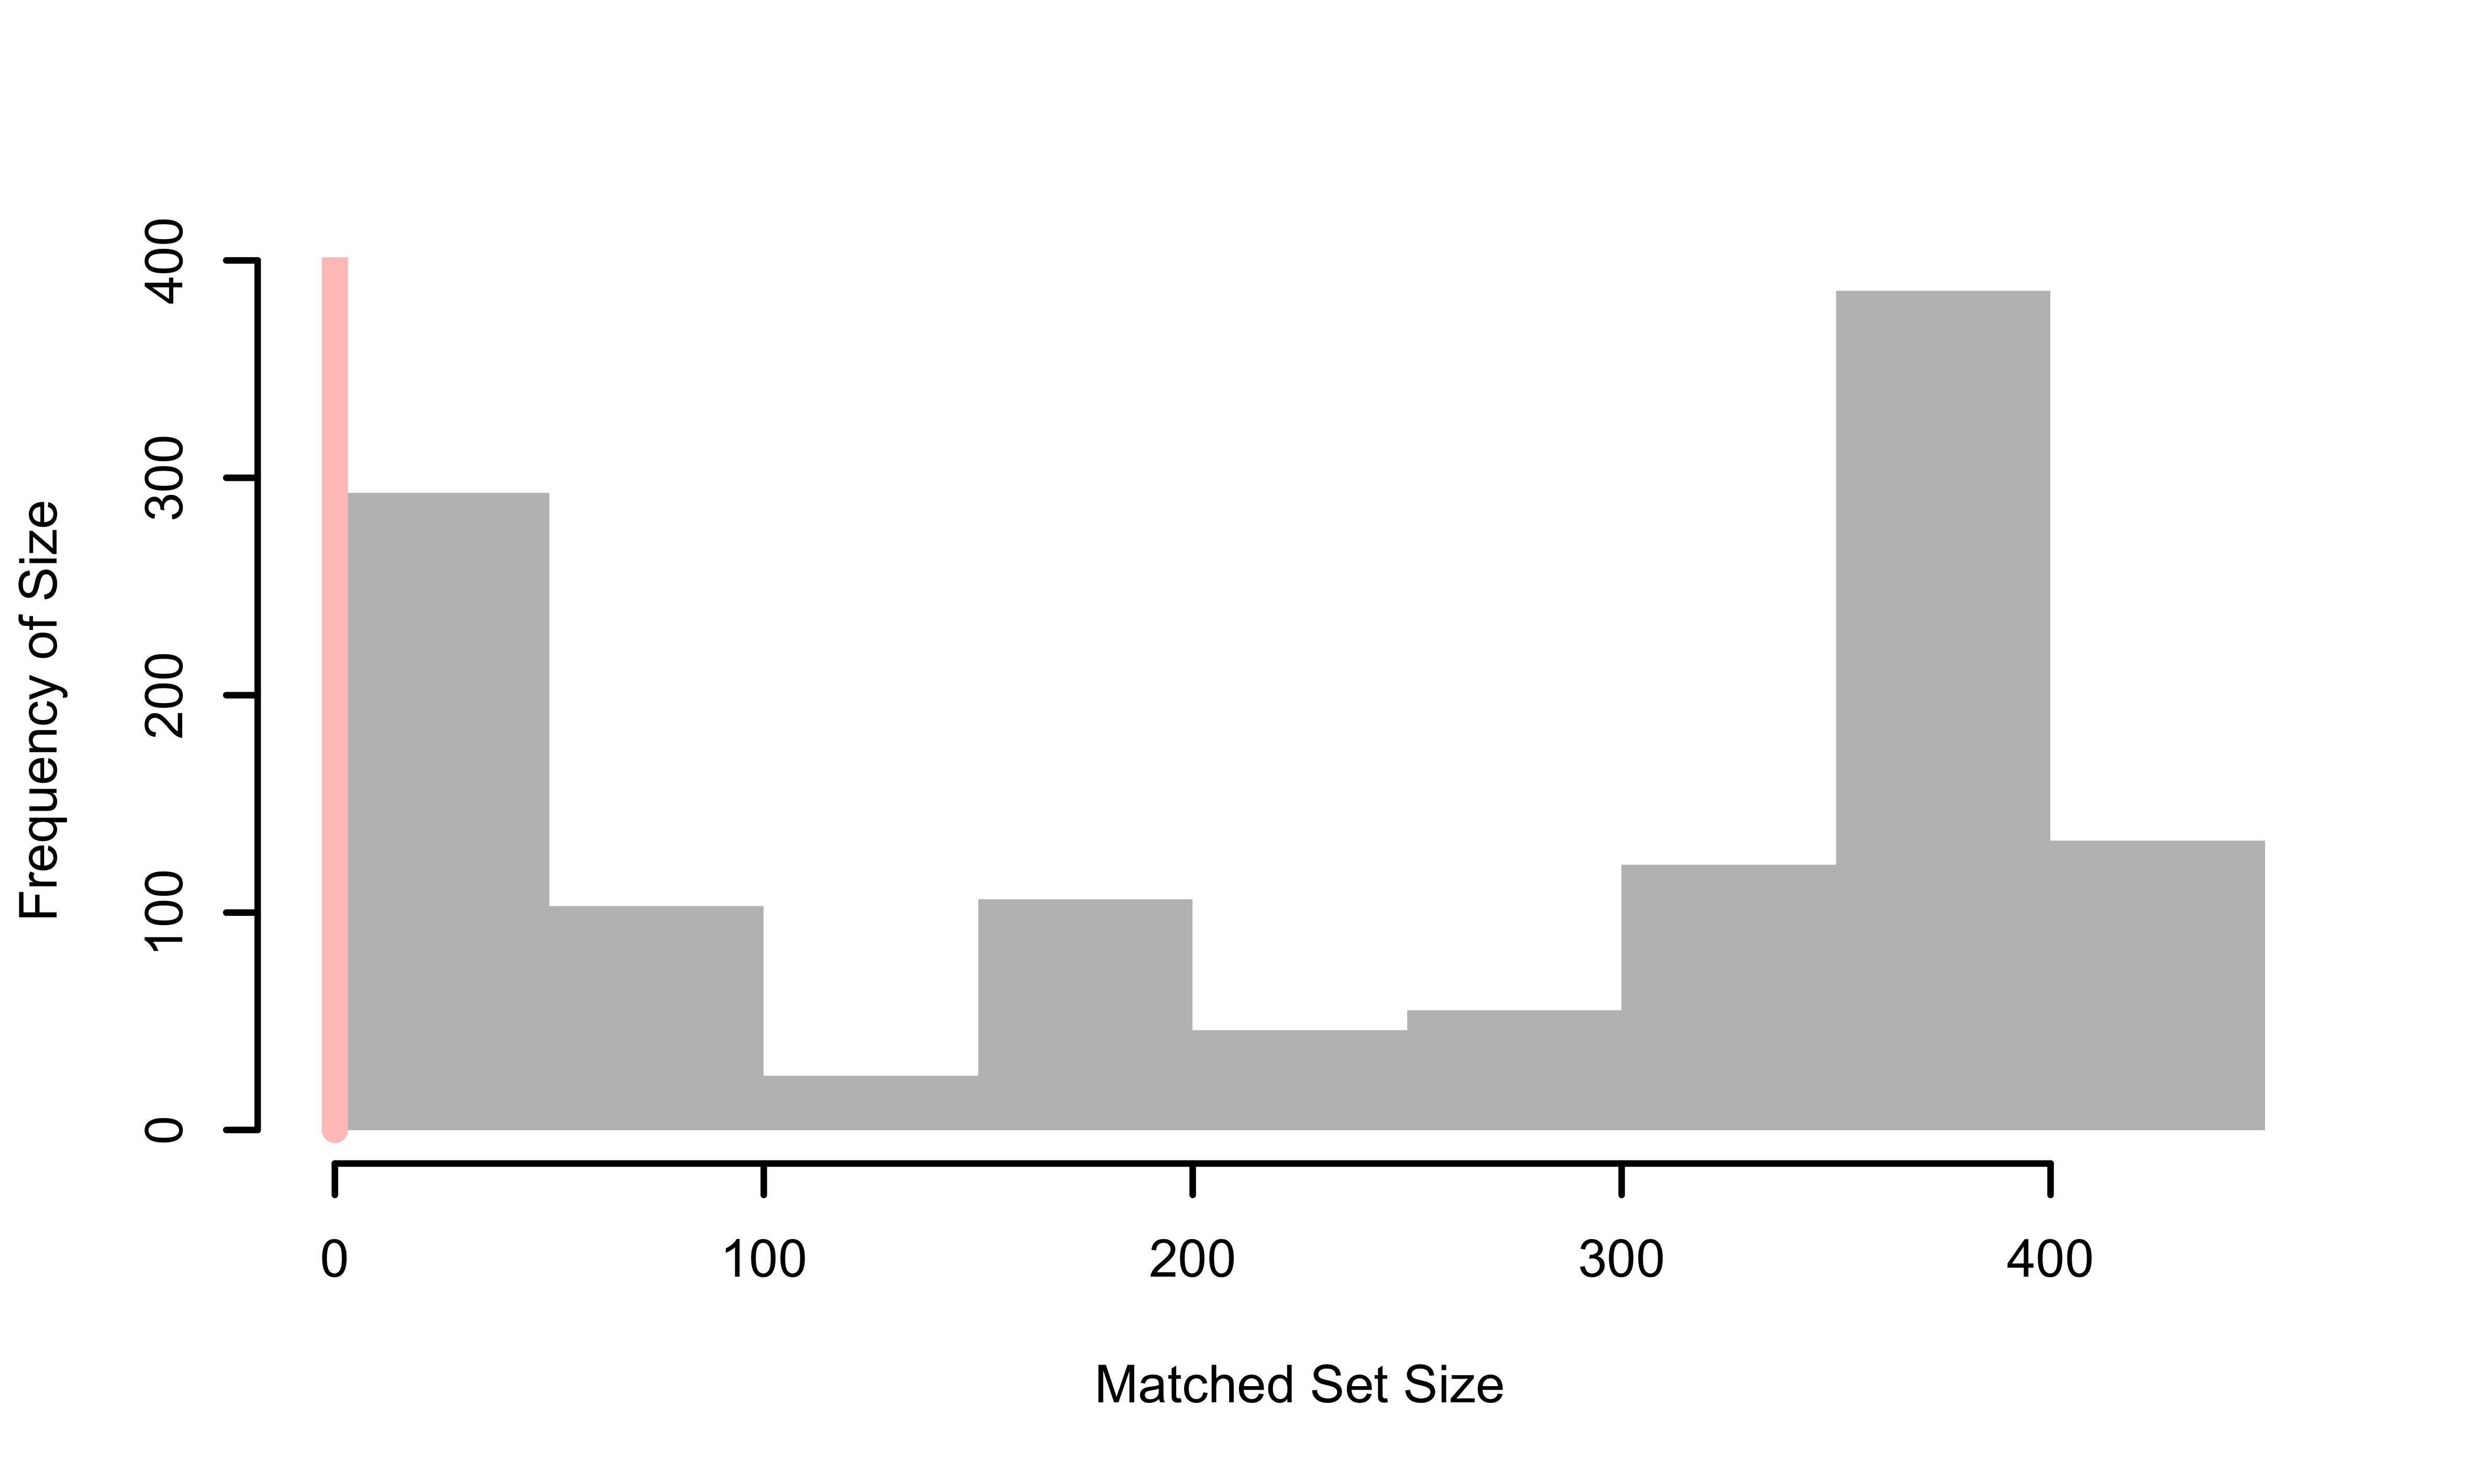
\includegraphics[width=0.8\linewidth]{\figdir/hist_matchset_size.png}
    \label{fig:hist_matchset_size}

    \fignote{\textwidth}{In the first step of the matching proceedure, each
        user gets assigned a set of potential control users that share the same
        treatment history for a specified number of periods before the user
        signs up to teh app (6 months, in our baseline specification), but that
        do not sign up themselves for a specified number of periods after the
        treatment user has signed up (another 6 months, in our baseline
        specification). The figure shows the distribution of the sizes of these
        sets of potential control users. The pink vertical bar on the left
    shows to count of users for whom no control users cound be found.}

\end{figure}

\begin{figure}[htpb]
    \centering
    \caption{Covariance balance}%
    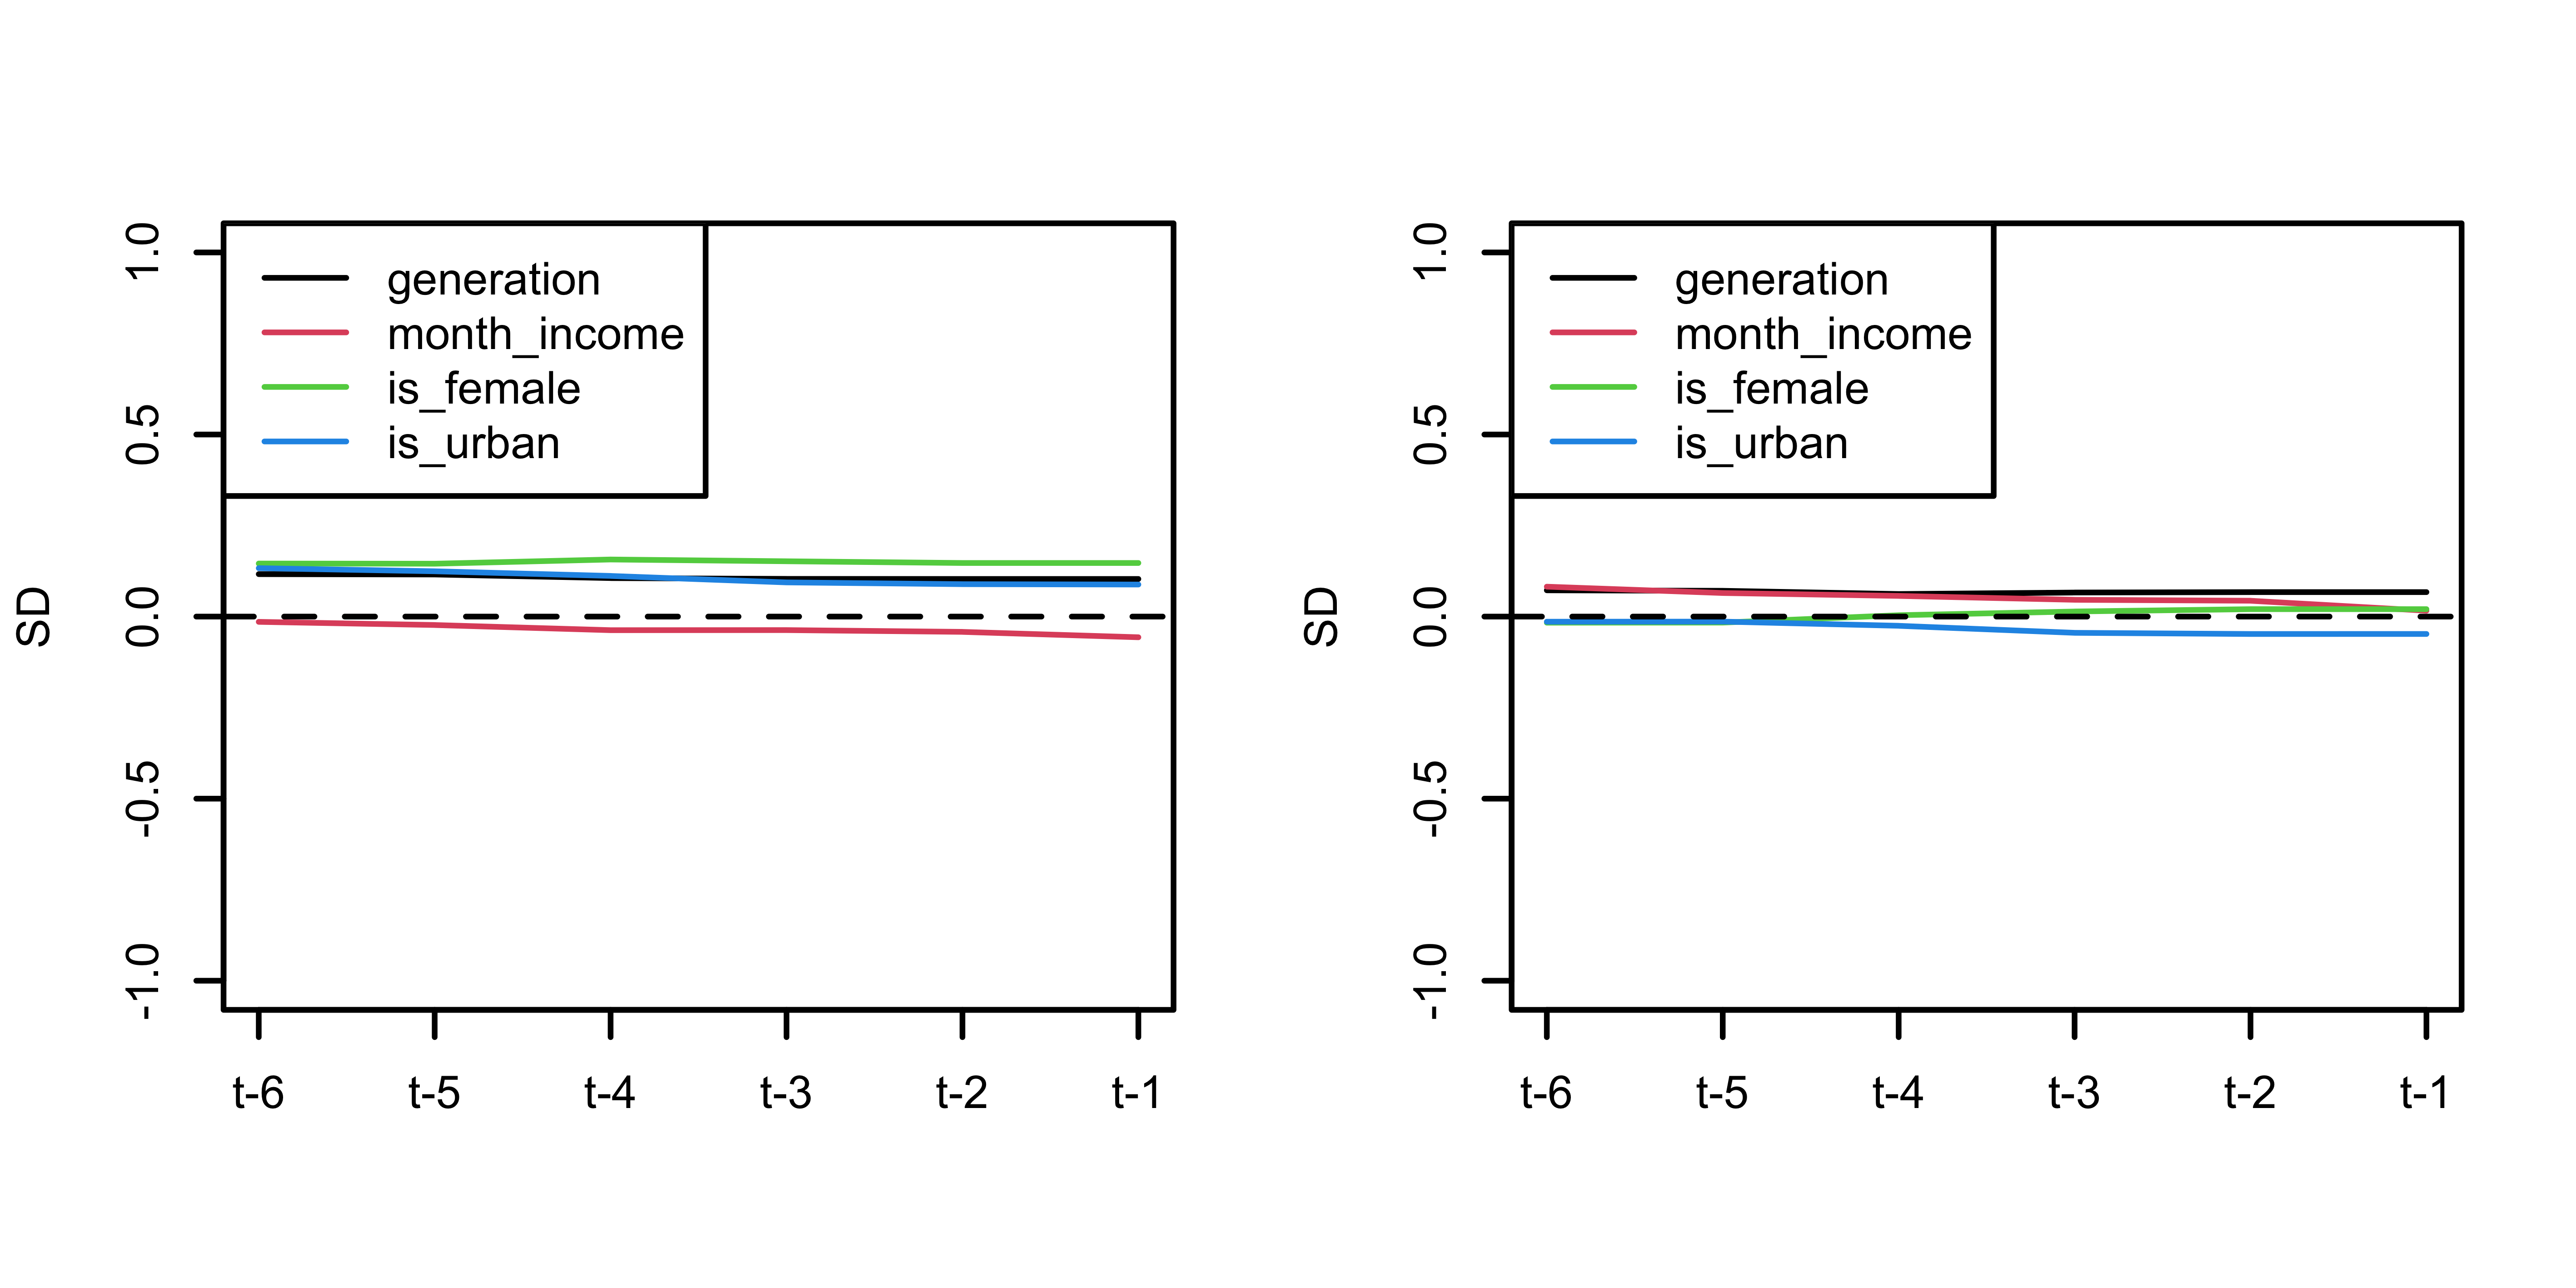
\includegraphics[width=0.8\linewidth]{\figdir/covar_balance.png}
    \label{fig:covar_balance}

    \fignote{\textwidth}{Average covariate standard deviation between treatment and
        control units for each pre-treatment period using the entire set of
        potential controls on the left and, on the right, the refined set of
        controls, which, in our baseline specification, consists of the nearest
        neighbour match based on the propensity score.}

\end{figure}

\begin{figure}[htpb]
    \centering
    \caption{Matching estimates}%
    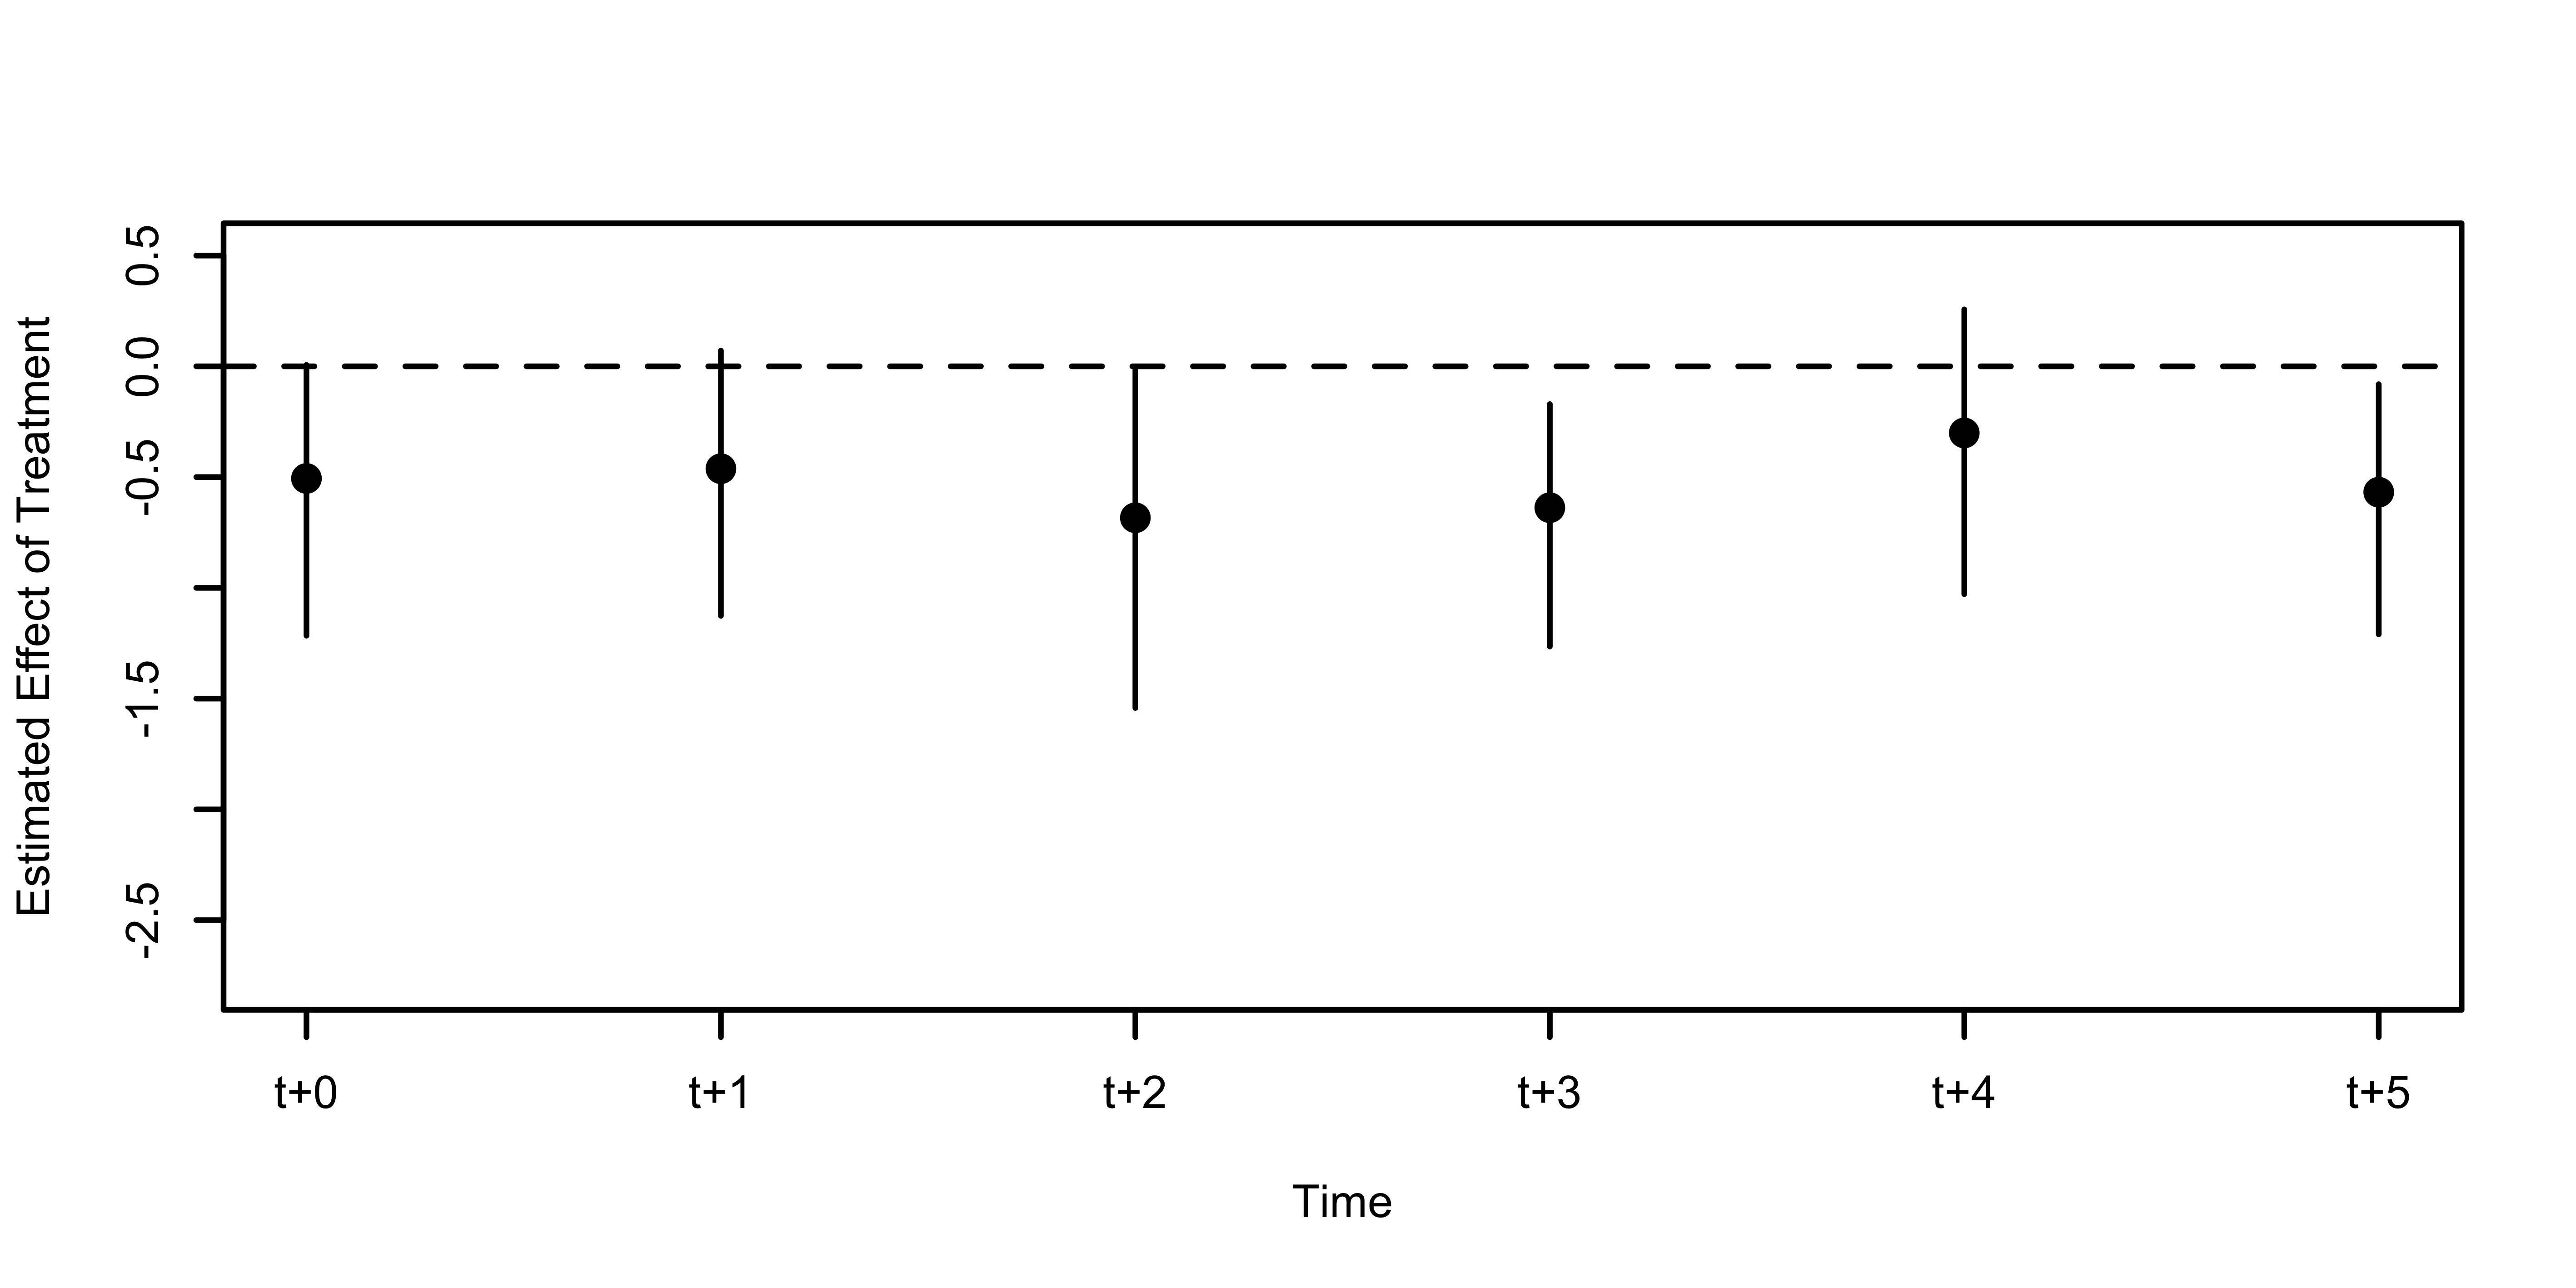
\includegraphics[width=0.8\linewidth]{\figdir/match_estimates.png}
    \label{fig:match_estimates}

    \fignote{\textwidth}{}

\end{figure}

Is estimate causal?
\begin{itemize}
    \item \citet{king2006dangers} show that there are four sources of bias
        (ommitted variable, posttreatment, interpolation, extrapolation).
    
    \item Discuss each in turn to argue that effect is causal (for our population
        of interest, which are people signing up to MDB). 
\end{itemize}


\subsection{Code access}%
\label{sub:code_access}

We provide links to code that creates key elements of the paper such as
variable definitions and sample selection directly in the relevant places in
the paper so they can be accessed conveniently. The links are indicated with
the GitHub logo, \faGithub. The hope is that this helps the
curious reader clarify questions about subtleties they might have while reading
the paper. The complete projects GitHub repo is at
\href{https://github.com/fabiangunzinger/mdb\_eval}{https://github.com/fabiangunzinger/mdb\_eval}.


